% use the base acmart.cls
% use the sigplan proceeding template with the default 10 pt fonts
% nonacm option removes ACM related text in the submission. 
\documentclass[sigplan,nonacm]{acmart}
\usepackage{csvsimple}
\usepackage{subcaption}

\newcommand{\fixme}[1]{\textcolor{red}{#1}}
\newcommand{\todo}[1]{\textcolor{red}{TODO:\ #1}}
\newcommand{\fullname}{More Exact FPGA Technology Mapping with E-Graphs}
\newcommand{\shortname}{E-Pack}
\newcommand{\metric}{12\% fewer LUTs}
\newcommand{\fmetric}{45\%}
\newcommand{\nimproved}{45}
\newcommand{\nbenchmarks}{99}
\newcommand{\B}{\mathbb{Z}_{2}}
\newcommand{\Bk}{\mathbb{Z}_{2}^{k}}
\newcommand{\Bx}[1]{\mathbb{Z}_{2}^{#1}}

% enable page numbers
\settopmatter{printfolios=true}


\begin{document}

\title{\fullname}

\begin{abstract}
    FPGA technology mapping is a well-studied problem and has been an area of
    interest in EDA tool design for decades. In most respects, the computational
    complexity of technology mapping is understood, and heuristic algorithms have
    been successfully employed to mitigate compile times while maintaining high QoR
    (quality of results). As transistor scaling comes to an end within the coming
    years, logic synthesis tools will become more of a bottleneck in the design of
    high performance accelerators. As a solution, we introduce E-Pack, an e-graph
    driven technology mapper that can better span the wide gap between SAT-based
    exact synthesis and heuristic cut enumeration techniques. We show that E-Pack
    can synthesize circuits with \metric{} on average---without ever
    increasing circuit depth. We also provide an empirical analysis of the runtime
    of E-Pack and show that it is still practical for large designs. Finally, we
    demonstrate that our compiler infrastructure is reusable, and future work can
    use our compiler for RTL equivalence checking or auditing the QoR of synthesis
    tools.
\end{abstract}
\maketitle % should come after the abstract

\section{Introduction}\label{sec:intro}
Given the complexity of modern electronic systems, a high degree of automation
is required to develop custom hardware within sensible timelines. At the
highest level, FPGA and ASIC design flows can be split into logic synthesis and
physical design (e.g., floorplanning placement and routing). This division of
work produces suboptimal designs, and neither are the individual synthesis
steps locally optimal on their own. However, circuit minimization problems in
general are NP-Hard~\cite{logicmin,twolevellogic}, and modern EDA flows bring
compile times down to the human timescale while maintaining acceptable quality
of results (QoR).

With the end of Dennard scaling and Moore's Law fading, the quality of logic
synthesis becomes more important. Hence, future synthesis tools will need to
expand the design spaces they explore and find more optimal solutions. Still,
finding provably optimal circuits is computationally intractable. In this
paper, we introduce how FPGA technology mapping can be augmented with e-graph
data structures to find \textit{more} exact solutions, without significantly
increasing compile times.

Technology mapping is the hand-off between logic synthesis and physical design.
It converts the abstract Boolean logic into a network of circuit elements that
belong to the target cell library. For FPGAs, the primary target cell is the
lookup table (LUT). Since every $k$-LUT can be re-programmed to satisfy any $k$
input boolean function, FPGA technology mapping has an unmistakably large
solution space. Whether the circuit is optimized for latency or area, most FPGA
tools approach technology mapping as a graph covering problem~\cite{flowmap,
    daomap, attmap, imap}. In the literature, a group of circuit nodes implemented
by a $k$-LUT is called a $k$-feasible cut of logic, and the generation of all
cuts is called cut enumeration. These structural mapping techniques rely on the
topology of the input circuit, and hence they are prone to \textit{structural
    bias}.

In contrast, functional mappers attempt to decompose the Boolean functionality
into smaller sub-functions which can be realized by $k$-LUTs. Such mappers are
a more exact approach, and often use SAT solvers to drive
synthesis~\cite{satmap,satmap2}. Other works employ Boolean matching to speedup
of technology mapping by identifying known Boolean
structures~\cite{boolmatch,fastboolmatch}. However, exact synthesis tools
cannot be scaled past tens of gates. As a consequence, cut enumeration and
functional mapping lie on two different extremes. The former is fast but
limited by the input structure, while the latter is unbiased but fundamentally
unscalable.

For this reason, we propose an e-graph driven technology mapper than can better
span the time-QoR spectrum. Equality graphs, referred to as e-graphs, are a
data structure which use union-find operations to compactly represent abstract
equivalence relations~\cite{eggpaper}. Whereas typical optimizing compilers
apply a greedy sequence of transformation passes, e-graphs rewrite terms
iteratively in a nondestructive fashion. Our work seeks to evaluate the
suitability of e-graphs for logic synthesis, specifically for technology
mapping to FPGAs. By using the output mappings of RTL synthesis tools as an
initial solution, we can use e-graphs to incrementally explore more compact
circuit topologies.

To that end, we propose \shortname{}: a tool for repacking FPGA netlists into
more compact forms---without increasing circuit depth. Our results show many
benchmarks, big and small, which synthesize to significantly fewer LUTs over
vendor EDA tools. To that end, our work makes the following contributions:

\begin{itemize}
    \item We formulate an intermediate language and set of e-graph rewrite rules that can
          explore circuit topologies that heuristic approaches miss.
    \item We evaluate our compiler against \nbenchmarks{} benchmarks combined from three
          sources: EPFL~\cite{epflbench}, ISCAS'85~\cite{iscasbench}, and
          LGSynth'91~\cite{lgsynthbench}. The results show improvements in LUT count
          without significant increases to compile time.
    \item Finally, \shortname{} is packaged as a Verilog-to-Verilog tool that can be
          dropped into existing RTL flows.
\end{itemize}

Before elaborating on our methodology and experimental setup, we first discuss
related ideas in technology mapping and e-graph driven compilers. Then, the
results section illustrates the typical reduction in LUT count our tool
achieves without increasing circuit depth. Lastly, we discuss the future work
of our compiler.
\section{Background}\label{sec:background}
\todo{explain background}
% Logic Synthesis

% Difficulty of the FPGA Mapping problem

% Formal Properties of E-Graphs


\section{Related Work}\label{sec:relatedwork}
% Related work todo
% - dsd
\subsection{LUT Packing}\label{sec:relatedwork:fpga}
FPGA technology mapping converts abstract RTL logic into a netlist of lookup
tables (LUTs). Due to the computational complexity of this problem, most
implementations avoid restructuring the input logic and are essentially graph
covering algorithms. Where competing implementations vary, however, is the set
of heuristics they use to guide optimization. Broadly speaking, FPGA LUT
packing can be divided into architecture-specific and architecture-nonspecific
optimizations. Architecture-specific LUT packing encapsulates optimizations
that reduce routing congestion by more efficiently using intra-CLB routing
resources. Examples include mapping dual-output functions to fractured
LUTs~\cite{fraclut} or using dedicated multiplexers to implement functions with
more than 6 inputs~\cite{ug574}.

In contrast, architecture-nonspecific LUT packing is more general as it
attempts to mitigate the structural bias of the input logic. As an example,
AGDMap~\cite{adaptdecomp} decomposes simple logic gates with large fanin to
enable the exploration of better graph coverings. However, structural bias can
take on many forms. For instance, FlowMap~\cite{flowmap} cites that the
non-monotone clustering of logic is the fundamental difficulty of LUT-based
technology mapping. In other words, a $k$-feasible cut of logic may contain
subcuts that are \textit{not} $k$-feasible. Overcoming bouts of non-monotone
clustering requires a more elaborate cut-selection algorithm, and our work lays
the foundation for a formal, reasoning-based approach to the problem.

\subsection{E-Graph Superoptimization}\label{sec:relatedwork:egraph}
Equivalence graphs (e-graphs) are a data structure originally conceived to
facilitate automated proof generation~\cite{eggpaper, eqsat}. For example,
e-graphs can be used to rewrite mathematical expressions~\cite{egraphmath} or
for automated reasoning about functional programs~\cite{cclemma}. In recent
years, e-graphs and equality saturation have enjoyed renewed popularity within
the compilers field. Equality saturation is useful for optimizing compilers,
because it defers greedy program transformations. Extracting solutions from
saturated e-graphs can result in more optimal---sometimes provably
optimal---programs. In contrast, traditional compilers use a pass pipeline
architecture which suffers from a \textit{phase-ordering problem}. In other
words, there is never an ordering of transformation passes that is optimal for
all input programs. This is a deep-rooted issue in compiler design, but the
problem is particularly consequential for hardware design. Several recent works
use e-graphs to improve upon typical optimizing compiler architecture.

SEER~\cite{seer} uses e-graphs to optimize the data-level and pipeline
parallelism of control flow in high-level synthesis (HLS) programs.
IMpress~\cite{impress} also uses e-graphs at the HLS level, optimizing the
muliplication of large bit-width integers. At a lower level,
ROVER~\cite{rover,roverbl,egraphconstraints} rewrites arithmetic data paths at
the word and bit levels. ROVER straddles the RTL and physical level of
abstraction, making it more general purpose than IMpredss. In any case, the
work which is most similar in its goals to ours is E-Syn~\cite{esynth}. E-Syn
rewrites the Boolean algebra of a circuit using known properties like De
Morgan's laws and the consensus theorem. Ultimately, E-Syn performs its
optimizations during technology-independent synthesis steps, whereas
\shortname{} applies as a post-processing step \textit{after} technology
mapping. Furthermore, \shortname{}'s rewriting system models the netlist in
terms of total functions, rather than as expressions over a Boolean algebra.
\section{E-Graph Construction}\label{sec:rewrites}
As an overview, an e-graph is built by accumulating new equivalence relations
through the iterative rewriting of terms. Rewrite rules define the equivalence
relations in full generality by designating a search pattern of terms to
rewrite. This prompts the creation of a grammar that can represent the
structure of electronic circuits and lends itself well to pattern matching. As
an example, one can write De Morgan's laws as rewrite rule:

\begin{lstlisting}
(NOT (AND x y)) => (OR (NOT x) (NOT y))
\end{lstlisting}

The left-hand side is the search pattern, and the right-hand side describes how
to apply the rewrite to the pattern. Rewrites must be merged back into the
union-find data structure, so this is an iterative process. In the following
subsections, we will define our netlist representation, \texttt{LutLang}, and
the accompanying equivalence relations. Formalizing the meaning of FPGA
netlists is critical to both ensuring correctness and finding deeper insight
into the structure of our rewrite rules under composition.

\subsection{\texttt{LutLang} Representation}\label{sec:rewrites:lutlang}

Input Verilog netlists are converted to our internal format, called
\texttt{LutLang}, which is compatible with e-graph structures. When printed to
text, \texttt{LutLang} takes on a Lisp-like syntax and our rewrite rules are
written in such style. As an example, a 2-LUT cascaded into a 3-LUT is written
as follows:

\begin{lstlisting}
(LUT G x2 x3 (LUT F x0 x1))
\end{lstlisting}

\texttt{G} and \texttt{F} are the truth-tables of the LUTs.
We also call them the \textit{program} or \textit{function} interchangeably.
Since $k \leq 6$, truth tables are stored as 64-bit integers, but we analyze them as total functions $F: \Bk \rightarrow \B$.
To clarify notation, $\mathbb{Z}_2 = \mathbb{Z}/2\mathbb{Z} = \mathbb{B} = \{0,1\}$.
To that end, the denotational semantics $\llbracket \cdot \rrbracket : \texttt{LutLang} \rightarrow \mathbb{Z}_2$ of a LUT is simply applying its Boolean inputs to the function:

\begin{equation}
    \llbracket \texttt{(LUT F x0 x1)} \rrbracket = F(\llbracket \texttt{x0} \rrbracket, \llbracket \texttt{x1} \rrbracket)
\end{equation}

\begin{figure}
    \centering
    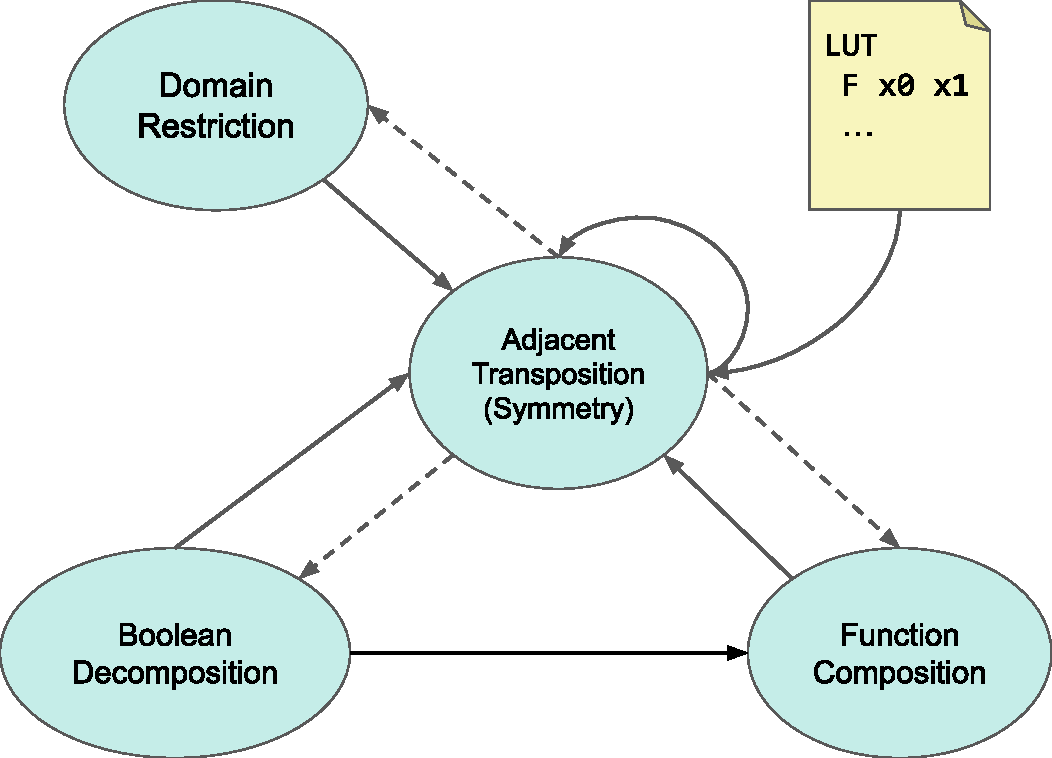
\includegraphics[width=0.47\textwidth]{img/rewrites.pdf}
    \caption{Transition diagram of rewrite rules. A solid arrow means that the application of the source rule always becomes an instance of the target rule.}\label{fig:rewrites}
\end{figure}

\subsection{Simplifying Degenerate LUTs}\label{sec:rewrites:degen}

\textbf{Definition:} A LUT's configuration $F : \Bk \rightarrow \B$ is \textit{degenerate} if there exists a Shannon expansion $F = x_i \cdot F_{x_i} + \overline{x_i} \cdot F_{\overline{x}_i}$
such that $F_{x_i} = F_{\overline{x}_i}$ for some input position $i \in \{ 0, \ldots, k -1\}$. In other words, $F = F_{x_i} = F_{\overline{x}_i}$.

The output of a degenerate LUT is not dependent on one of its inputs. Hence, it
can be rewritten into a LUT which uses fewer inputs. This rule is applied by
computing the Shannon expansions of LUTs and checking for equivalence. As an
example, the rule takes on the following form in pseudocode for $k=3$:

\begin{lstlisting}
(LUT F x0 x1 x2) => (LUT F' x0 x1)
    if F(x0, x1, false) == F(x0, x1, true)
    where F'(x0, x1) := F(x0, x1, true)
\end{lstlisting}

On the left of \texttt{=>} is the \textit{search pattern}. The right-hand side
of the rule is the \textit{application}. One rule is instantiated for each LUT
size $k =1$ through 6. One should notice that LUTs which are constant functions
are also handled by this rule. Since this rule is computationally expensive, it
is applied greedily as a pre-processing step before the e-graph is built. None
of the other rewrite rules create degenerate LUTs, so this has no impact on
results.

\subsection{Partial Application}\label{sec:rewrites:application}
A LUT with a constant input can be partially evaluated to a LUT with one less
input. This rule is similar to the last. It computes the Shannon expansion
along the constant variable and chooses the cofactor that matches the state of
the constant input. One could show that applying this rule greedily in
combination with the previous one is equivalent to constant propagation. As an
example, the pseudocode for $k=3$ is written as follows:

\begin{lstlisting}
(LUT F x0 x1 false) => (LUT F' x0 x1)
    where F'(x0, x1) := F(x0, x1, false)
\end{lstlisting}

\subsection{LUT Symmetries}\label{sec:rewrites:symmetry}

The semantics of LUTs should not depend on the order of their inputs. If two
LUTs have permuted inputs but are otherwise functionally identical, they should
belong to the same e-class in the graph. That is, \mbox{\texttt{(LUT F .. xi ..
        xj ..)}} is semantically equivalent to \mbox{\texttt{(LUT G .. xj .. xi ..)}}
if and only if $G = F \odot \sigma^{-1}$, where $\sigma \in S_k$ is the
permutation applied to the inputs.

\begin{proof}
    $\odot$ is a right-action defined for the sake of permuting the inputs to a function before they are applied:
    \begin{equation*} \odot : \big (\Bk \rightarrow \mathbb{Z}_2 \big ) \times S_k \rightarrow \big (\Bk \rightarrow \mathbb{Z}_2 \big ) \end{equation*}
    \begin{equation*} F \odot \sigma : (x_0, x_1, \ldots, x_{k-1}) \mapsto F(x_{\sigma(0)}, x_{\sigma(1)}, \ldots, x_{\sigma(k-1)}) \end{equation*}

    It is trivial to prove that this right-action is associative:
    \begin{align*}
        (F \odot \sigma_1) \odot \sigma_2 & = F(x_{\sigma_2(\sigma_1(0))}, x_{\sigma_2(\sigma_1(1))}, \ldots, x_{\sigma_2(\sigma_1(k-1))}) \\
        (F \odot \sigma_1) \odot \sigma_2 & = F \odot (\sigma_2 \circ \sigma_1)
    \end{align*}
    With this property, the rest follows directly:
    \begin{equation}
        F = G \odot
        \sigma \iff F \odot \sigma^{-1} = (G \odot \sigma) \odot \sigma^{-1} = G
    \end{equation}
\end{proof}

Therefore, we can conclude that $k$-LUTs have as much symmetry as can be
generated by the group $S_k$. The insight from this formal approach has two
main consequences. First, it precisely reveals how many e-graph rewrite rules
are needed to generate all the symmetries of a LUT. For any $k$-LUT with
program $F$, we need exactly as many rules as it takes to generate $F \odot
    S_k$. It is a well-known fact in algebra that the $k-1$ adjacent transpositions
generate $S_k$~\cite{sgroup}. Therefore, we can insert an e-graph rewrite rule
for each adjacent transposition. In total, there are $\sum_{k=2}^{6} (k-1) =
    15$ rules to encapsulate symmetry for every LUT size. The second consequence is
that every other rewrite rule can now be defined for one input position,
without loss of generality. This reduces the total number of rewrite rules,
making it easier to rationalize about the rule system and which types of
optimizations are reachable.

\subsection{Function Composition}\label{sec:rewrites:composition}

Cascaded LUTs can be packed into a single LUT, as long as the size of the cut
of logic has at most 6 leaf nodes. This is the crucial observation to LUT
packing. For instance, a circuit that implements $F(x_0, G(x_1, x_2))$ with two
2-LUTs can be rewritten as a 3-LUT that implements some $H(x_0, x_1, x_2)$. In
pseudocode, this would take on the following form:

\begin{lstlisting}
(LUT F x0 (LUT G x1 x2)) => (LUT H x0 x1 x2)
    where H(x0, x1, x2) := F(x0, G(x1, x2))
\end{lstlisting}

The search patterns \texttt{x0}, \texttt{x1} and \texttt{x1} can match any
node. They are not necessarily principal inputs, and hence can be outputs from
other LUTs. As a consequence, this rule can be chained together many times in
different orders to pack a sub-circuit into a single LUT. As an example, this
rule would match the two 4-LUTs in Fig.~\ref{fig:eg:bad} and combine them into
the single 4-LUT in Fig.~\ref{fig:eg:good}. Since the previous rule captures
LUT symmetry, we can write compositions for one specific input position,
without loss of generality. Therefore, we only need to sweep over the size of
the two LUTs in the search pattern. In total, there are $6 \cdot 6 = 36$ LUT
packing rules. When the cut of logic is larger than 6 leaves, the rule exits
gracefully and does not interfere with reaching equality saturation.

\subsection{LUTs with Domain Restrictions}\label{sec:rewrites:restrict}

\textbf{Definition:} A lookup table \texttt{(LUT F x0 x1 \ldots)} is
\textit{restricted} if $\llbracket \texttt{xi} \rrbracket = \llbracket \texttt{xj} \rrbracket$
for some $ i, j \in \{0, \ldots, k-1\}, \; i \neq j$. In other words, the
domain of the LUT is restricted.

The main advantage of using e-graphs is the compact way in which it represents
notions of equality. Whenever a new equivalence is found between two of the
inputs to a $k$-LUT, it can be rewritten with a $(k-1)$-LUT. We simply need to
define and compute $\texttt{restrict(F, i, j)}$ which maps $F : \Bx{k}
    \rightarrow \B$ to the domain-restricted $F \vert_{x_i = x_j} : \Bx{k-1}
    \rightarrow \B$. In pseudocode, the rewrite rule can be written as follows:

\begin{lstlisting}
(LUT F x0 x1 x1) => (LUT F' x0 x1)
    where F' := restrict(F, 1, 2)
\end{lstlisting}

Since rewrite search patterns already match `modulo' e-class, this rule is
automatically triggered when e-classes are merged. For instance, if the e-graph
proved in Fig.~\ref{fig:eg} that $A_i = B_i$ then all the LUTs would shrink by
one input---causing the next wave of rewrites to fire. Again, only one rule is
needed for each LUT size $k=2$ through 6, because LUT symmetry is represented
in the graph.

\begin{figure*}[tb]
    \begin{subfigure}{0.31\textwidth}
        \centering
        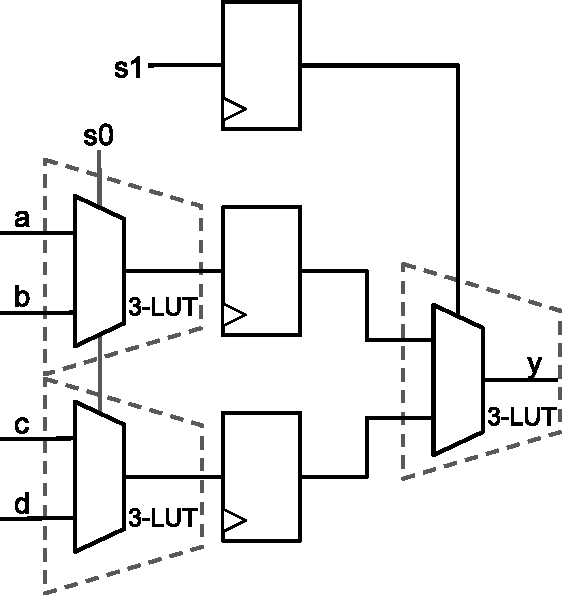
\includegraphics[width=0.88\textwidth]{img/mux_4_1.pdf}
        \caption{Three 3-LUT, three FF topology.}\label{fig:retiming:a}
    \end{subfigure}
    \begin{subfigure}{0.38\textwidth}
        \centering
        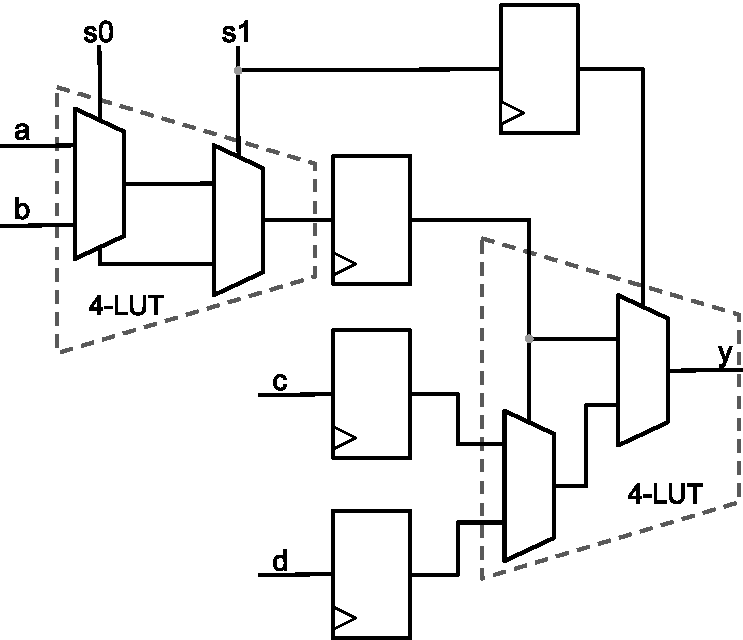
\includegraphics[width=0.9\textwidth]{img/mux_4_1_retime_dsd.pdf}
        \caption{Two 4-LUT, four FF topology.}\label{fig:retiming:b}
    \end{subfigure}
    \begin{subfigure}{0.30\textwidth}
        \centering
        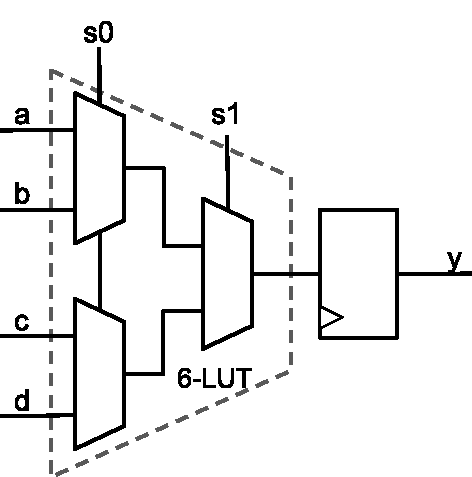
\includegraphics[width=0.84\textwidth]{img/mux_4_1_retime.pdf}
        \caption{One 6-LUT, one FF topology.}\label{fig:retiming:c}
    \end{subfigure}
    \caption{Three varying topologies for 4:1 MUX with pipeline register.}\label{fig:retiming}
\end{figure*}

\subsection{Functional Decomposition}\label{sec:rewrites:decomp}

Decomposing boolean functions and logic minimization in general is
NP-complete~\cite{logicmin}. Correspondingly, decomposing LUTs explodes the
size and build time of the e-graph. However, we can still define rewrites that
look for fully disjoint decompositions in one or more variables. This rule has
no structural element to search for, so it runs every time an e-class is
updated. Our implementation computes the Shannon expansion of a $k$-LUT's
function $F$ and checks that both cofactors are cognates in a loose sense. For
instance, given $k=3$ then it is true that for $G, H \in \B^2 \rightarrow \B$
that:

\begin{gather}
    F(x_0, x_1, x_2) = G(x_0, H(x_1, x_2)) \nonumber \\
    \Big\Updownarrow                       \nonumber \\
    F(x_0, x_1, x_2) = x_0 \cdot G_{x_0} (H(x_1, x_2)) +  \overline{x_0} \cdot G_{\overline{x}_0} (H(x_1, x_2))
\end{gather}

In practice, our implementation checks if either of the cofactors $G_{x_0}$ or
$G_{\overline{x}_0}$ are constant functions or if the cofactors are equivalent
up to complementation.

\subsection{Register Retiming}\label{sec:rewrites:retiming}

Register retiming is a purely structural rule, meaning it can be implemented
with a simple search and apply pattern. An example for $k=1$ would be written
as follows:

\begin{lstlisting}
(LUT F (REG x0)) <=> (REG (LUT F x0))
\end{lstlisting}

Unlike the other rules, this rule is searched for in both directions.
Figure~\ref{fig:retiming} illustrates an example of how register retiming can
compose with LUT rewrite rules to reduce LUT count and register count
simultaneously. In this case, the 3-LUTs implementing 2:1 multiplexers are
pushed across register boundaries. Since this logic happens to have a 6-LUT
packing and a two 4-LUT packing, we can explore a circuit topology that reduces
cell count (Fig.~\ref{fig:retiming:c}) or adjusts the delay paths
(Fig.~\ref{fig:retiming:b}). To best utilize register retiming, the e-graph
extraction technique must have some sense of timing information. Our e-graph
extractor is explained in the next section, but it should be noted that in our
experiments the area of LUTs and registers are weighted equally.
\begin{figure}
    \begin{subfigure}{0.47\textwidth}
        \centering
        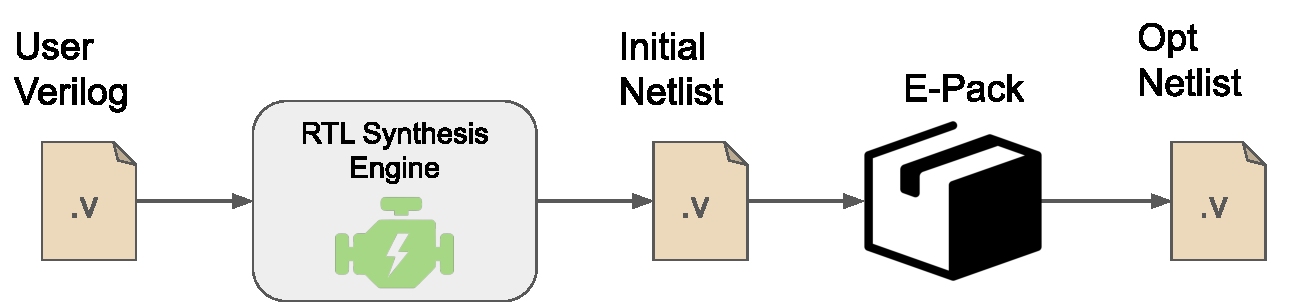
\includegraphics[width=\textwidth]{img/flow.pdf}
        \caption{The design flow integrating \shortname{} with existing RTL tools.}\label{fig:flow:rtl}
    \end{subfigure}
    \hfill\vspace{4mm}
    \begin{subfigure}{0.47\textwidth}
        \centering
        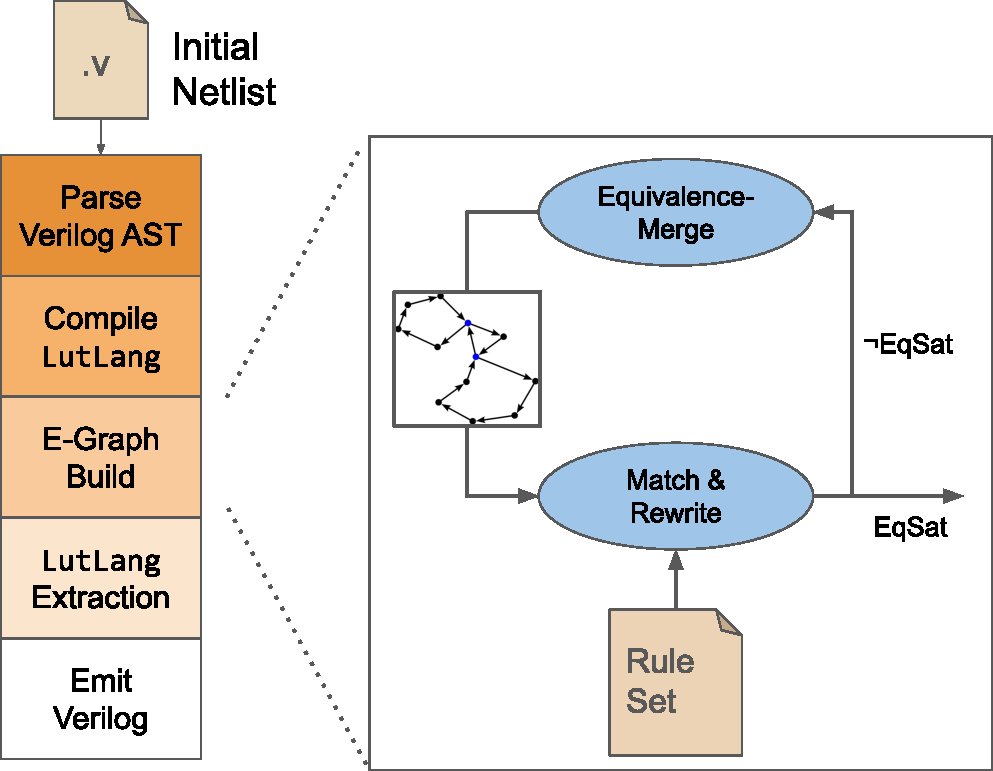
\includegraphics[width=\textwidth]{img/egraph.pdf}
        \caption{The compilation steps internal to \shortname{} Verilog tool.}\label{fig:flow:egraph}
    \end{subfigure}
    \caption{Diagrams of the top-level integration of \shortname{} into existing tool flows and internal compiler architecture.}\label{fig:flow}
\end{figure}

\section{Tool Flow}\label{sec:flow}

While constructing the e-graph is the crux of \shortname{}, there are several
other important components to consider in the full design flow. In order to
test our hypothesis, \shortname{} must be compatible with existing synthesis
flows, and the rewritten circuits must be verified. Fig.~\ref{fig:flow}
provides an overview on both the integration with existing RTL flows and the
internal compiler architecture. The following sections will describe each step
in more detail.

\subsection{Extraction}\label{sec:flow:extraction}
Regardless of whether equality saturation is achieved or not, the quality of
the output circuit still largely depends on the extraction technique used. In
short, \textit{extraction} is the process of selecting the ``best'' circuit
from the e-graph. Given that a saturated e-graph can contain hundreds of
thousands of e-nodes across tens of thousands of e-classes, a greedy extraction
algorithm is the most pragmatic. The greedy extractor iterates over the
e-classes, updating the cost of the cheapest e-node until the database of costs
no longer change. Whenever possible, our compiler uses the built-in
functionality of the egg e-graph Rust library~\cite{docsEgg}. However, e-graph
extraction itself is an ongoing research area~\cite{smoothe,
    sparsextract,esynth}, and future work should experiment with more capable
extraction algorithms. Aside from increases in compile time, better extraction
has the potential to raise the QoR yet another level. In any case, the greedy
cost of a LUT is always one plus the sum of the costs of its children nodes.
Further interactions between extraction and the rewrite rule set are further
explained in Section~\ref{sec:results:margin}.

\subsection{Verilog Support}\label{sec:flow:verilog}
In order for our compiler to be compatible with as many existing design flows
as possible, some level of Verilog support is necessary. Our compiler supports
a subset of Verilog 2001~\cite{verilog}, as required to represent structural
netlists. This includes support for non-ANSI C style module declarations,
wires, and module instantiations with named port connections. With Verilog
support, we are able to test \shortname{} with tool flows that use
Yosys~\cite{yosys} or Vivado~\cite{vivado}. On the backend, our compiler also
emits an updated Verilog netlist.

\subsection{Verification}\label{sec:flow:verification}
While formal verification is not the primary focus of this work, using e-graphs
as a formal reasoning tool helps to build trust in our synthesis results. In
fact, e-graphs were originally designed for automated theorem
proving~\cite{eggpaper}. Thus, constructing proofs that demonstrate equivalence
between the original and remapped netlist is a built-in feature of
\shortname{}. This technique is relatively slow, so we also use two other
independent sources of verification. For combinational netlists, our middle end
can do exhaustive functional testing. Lastly, we use Yosys~\cite{yosys} for its
SAT-driven equivalence checking capabilities. All in all, the mixed usage of
these verification techniques build confidence in the robustness of our
technology mapper built around e-graphs.
\section{Results}\label{sec:results}
Our experiments were carried out on a Red Hat 8 server hosting a Intel Xeon
Gold 6242 CPU. Since \shortname{} is written in Rust, it mostly uses the
built-in functionality of the egg library. The egg e-graph runner was ran in a
time-limited configuration, meaning there was no limit in the size of the
e-graph. Regardless, the median time to saturate a design was 9 seconds. As for
the benchmarks, \shortname{} was evaluated against circuits from three test
suites: EPFL~\cite{epflbench}, ISCAS'85~\cite{iscasbench}, and
LGSynth'91~\cite{lgsynthbench}. However, we also included an ALU and pipelined
multiplication module to test how our compiler behaves with increasing levels
of bit-parallelism and register pipelining. Finally, we measure how our
remapping optimizations influence CLB usage.

\begin{table}
    \centering
    \caption{Results of \nimproved{} improved benchmarks from ISCAS'85, LGSynth'91, and EPFL. The percent improvements use Vivado as the baseline.}\label{tab:results}
    \csvautobooktabular{data/results.csv}
\end{table}

\begin{figure}
    \begin{subfigure}{0.47\textwidth}
        \centering
        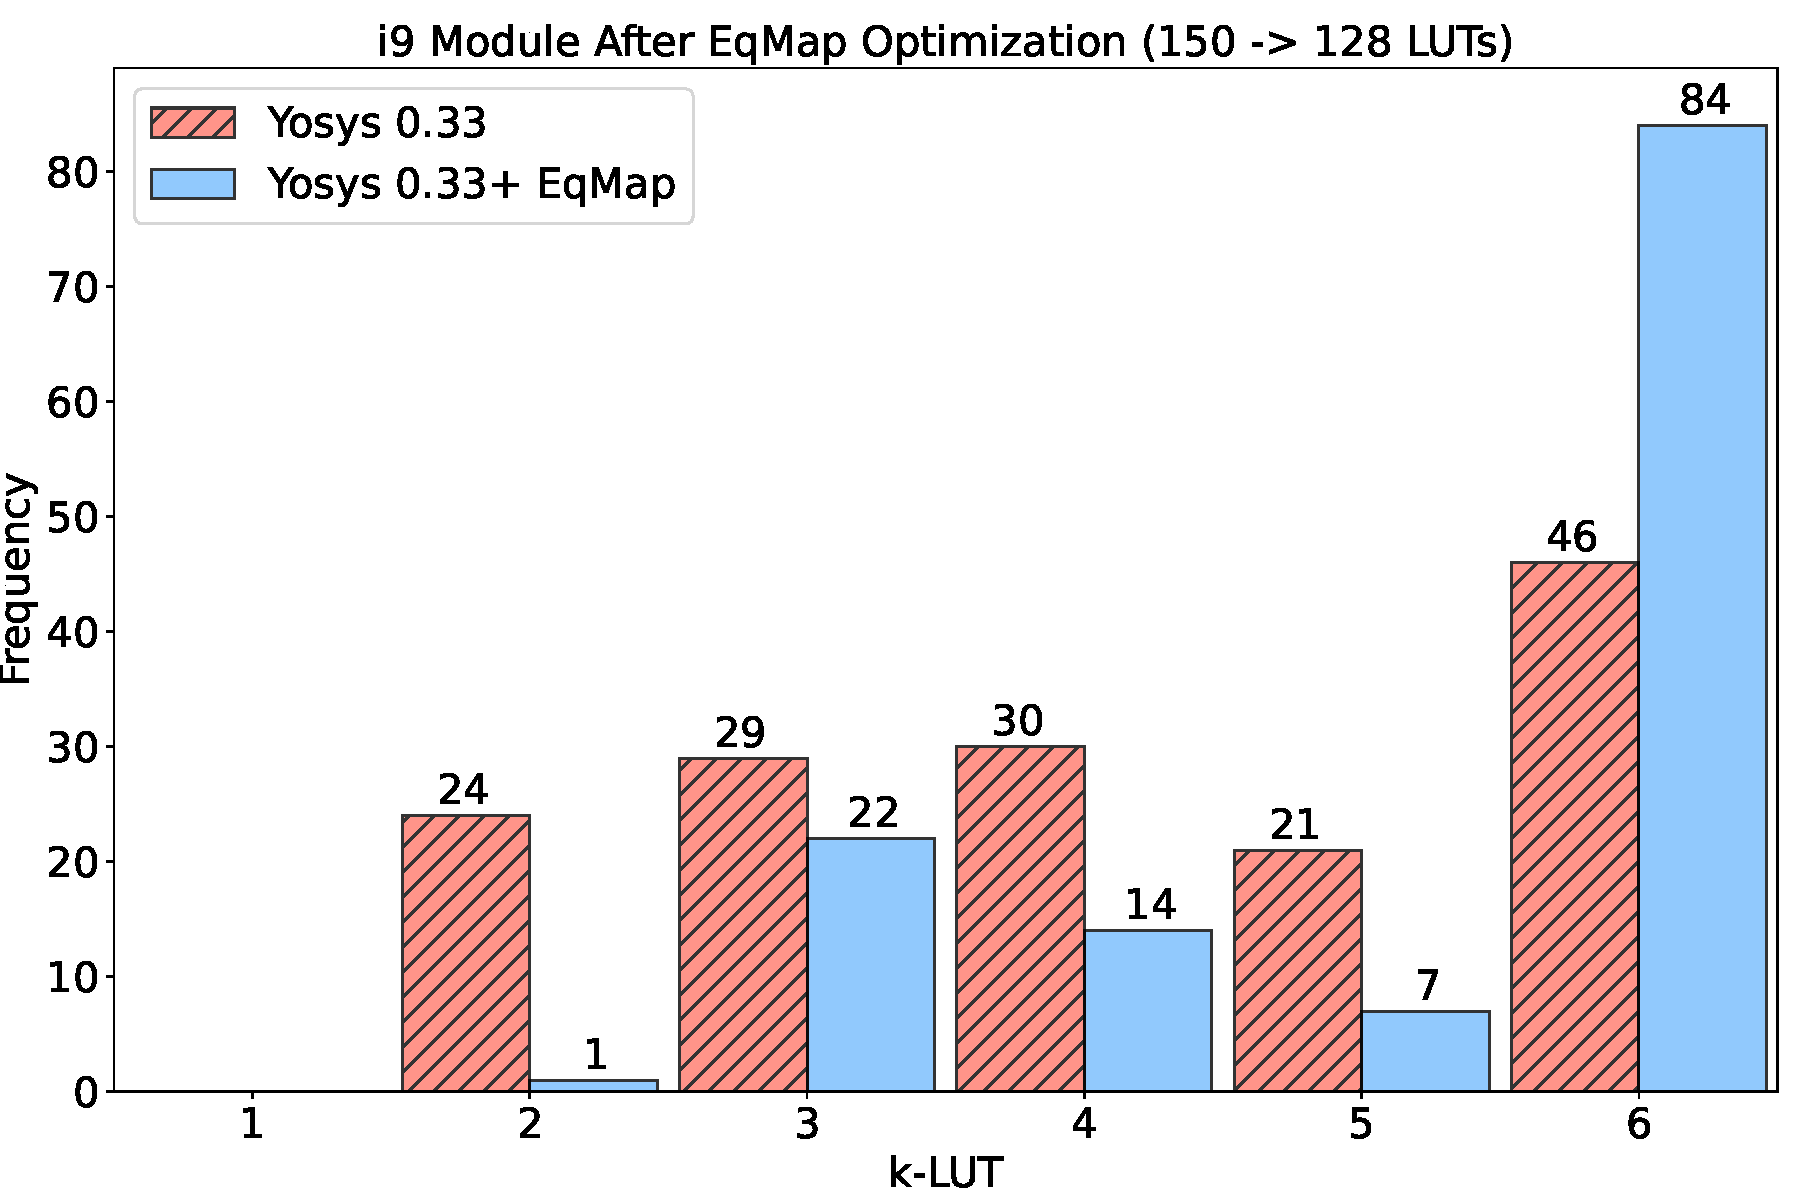
\includegraphics[width=\textwidth]{img/y33.pdf}
        \caption{Distribution of LUTs when using EqMap + Yosys 0.33.}\label{fig:histogram:y33}
    \end{subfigure}
    \hfill\vspace{4mm}
    \begin{subfigure}{0.47\textwidth}
        \centering
        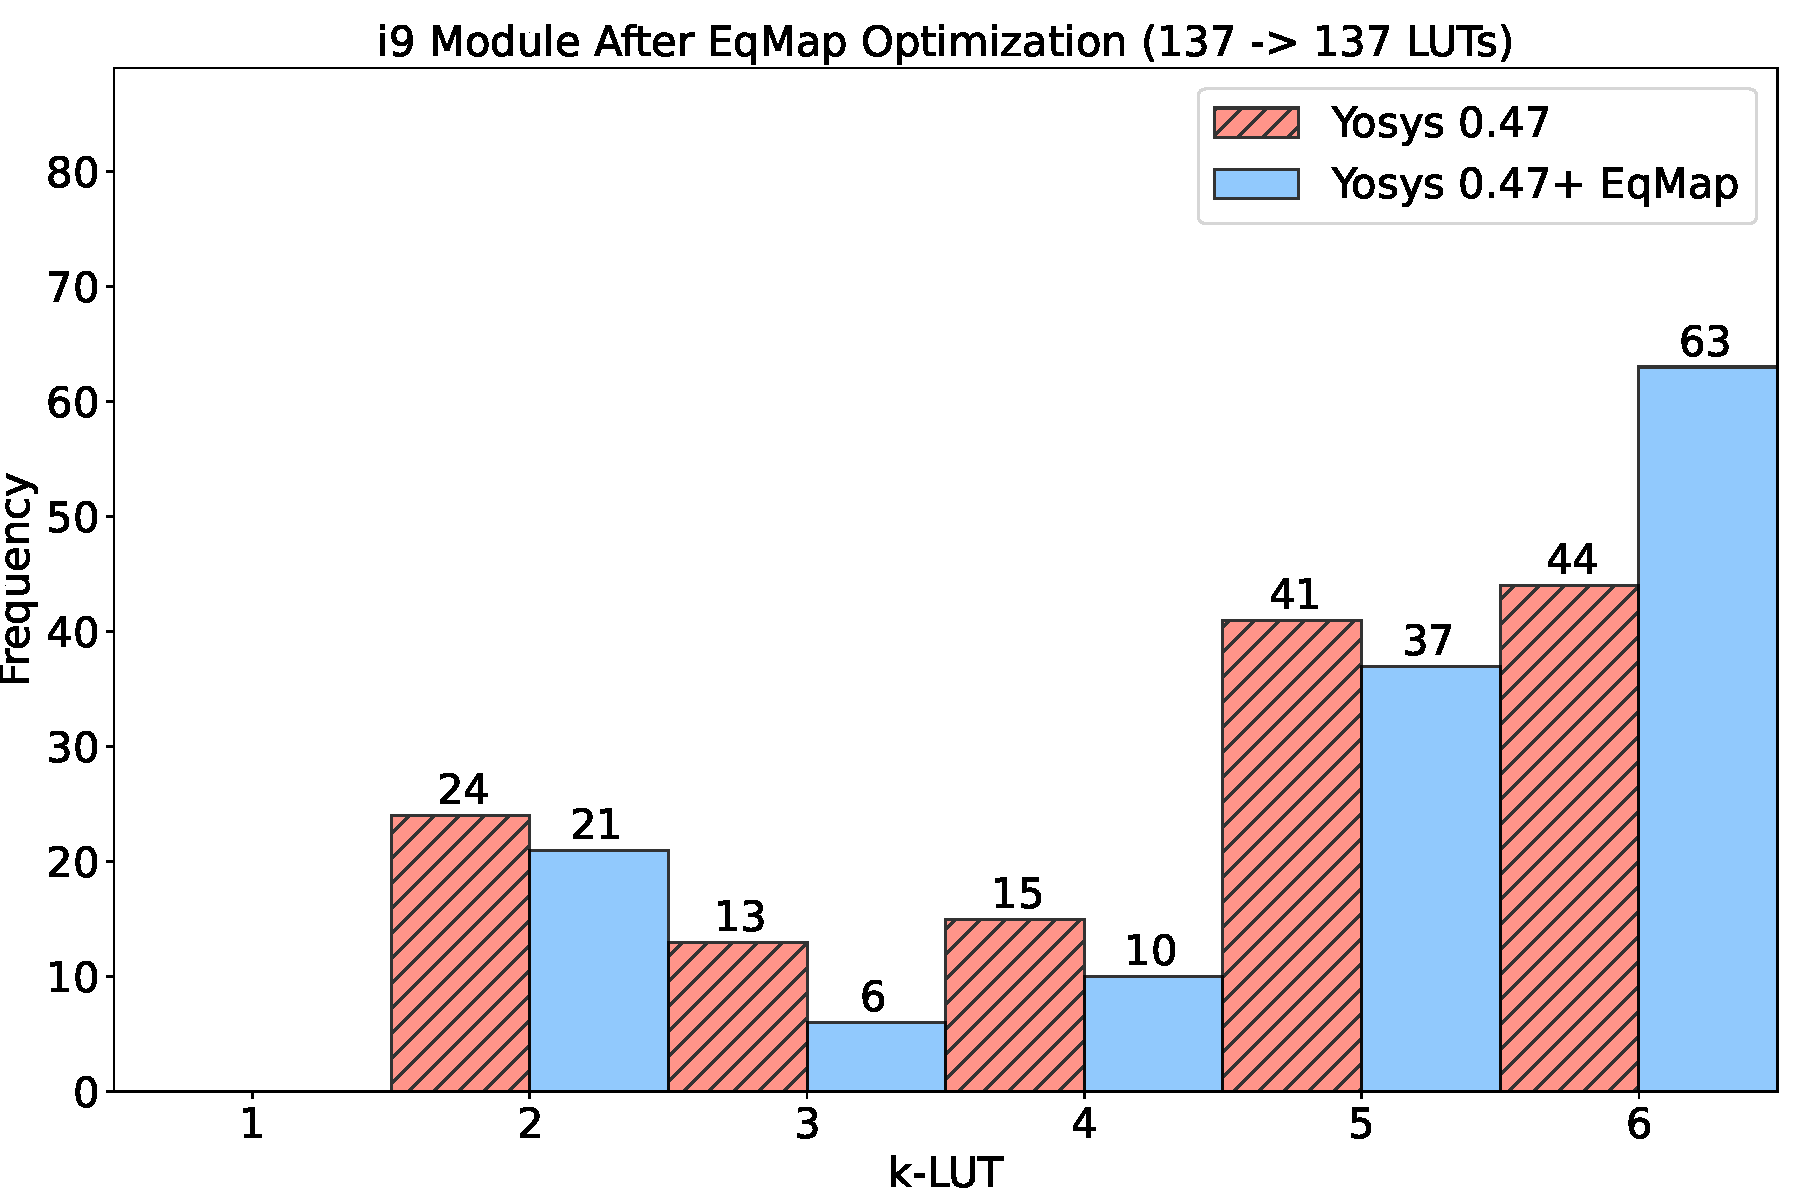
\includegraphics[width=\textwidth]{img/y47.pdf}
        \caption{Distribution of LUTs when using EqMap + Yosys 0.47.}\label{fig:histogram:y47}
    \end{subfigure}
    \caption{Yosys 0.47 maps `i9' with fewer LUTs than Yosys 0.33. However, remapping with EqMap causes the trend to invert.}\label{fig:histogram}
\end{figure}

\subsection{Benchmarking}\label{sec:results:benchmark}

We used a compilation of \nbenchmarks{} combinational benchmarks from three
academic sources to test LUT mapping ability. Among the combinational
benchmarks we tested, \shortname{} was able to reduce the LUT count \fmetric{}
of the time. On average, \shortname{} packed the netlists to \metric{}. The
results in Table~\ref{tab:results} list all the reduced LUT counts, sorted by
approximate design size. AMD/Xilinx Vivado 2024~\cite{vivado} was used as the
baseline synthesis tool. For the \shortname{} flow, Yosys~\cite{yosys} was used
to generate the initial mapped circuit. At a glance, circuits like `int2float,'
`c6288,` `adder,' and `square' have the most to gain from \shortname{}. These
circuits are all arithmetic in nature, and this pattern continues throughout
the rest of the results.

One result that is \textit{not} demonstrated by the table is the apparent
importance of the initial structure inputted to \shortname{}. We have not
eliminated all sources of structural bias, and hence our superoptimization tool
still occasionally gets stuck at a local minimum. Fig.~\ref{fig:histogram}
illustrates the issue by depicting the different distributions of $k$-LUT usage
by different tool flows. In short, an overly packed LUT network will fare worse
in attempts to superoptimize it. Future work will investigate which qualities
make an RTL synthesis engine work well with our tool versus ones that do not.
For example, \shortname{} optimized Yosys 0.33 netlists
(Fig.~\ref{fig:histogram:y33}) better than ones provided by Yosys version 0.47
(Fig.~\ref{fig:histogram:y47}). A future version of \shortname{} should
implement new rewrite procedures than can break out of these local minimums on
their own.

\begin{figure}
    \begin{subfigure}{0.47\textwidth}
        \centering
        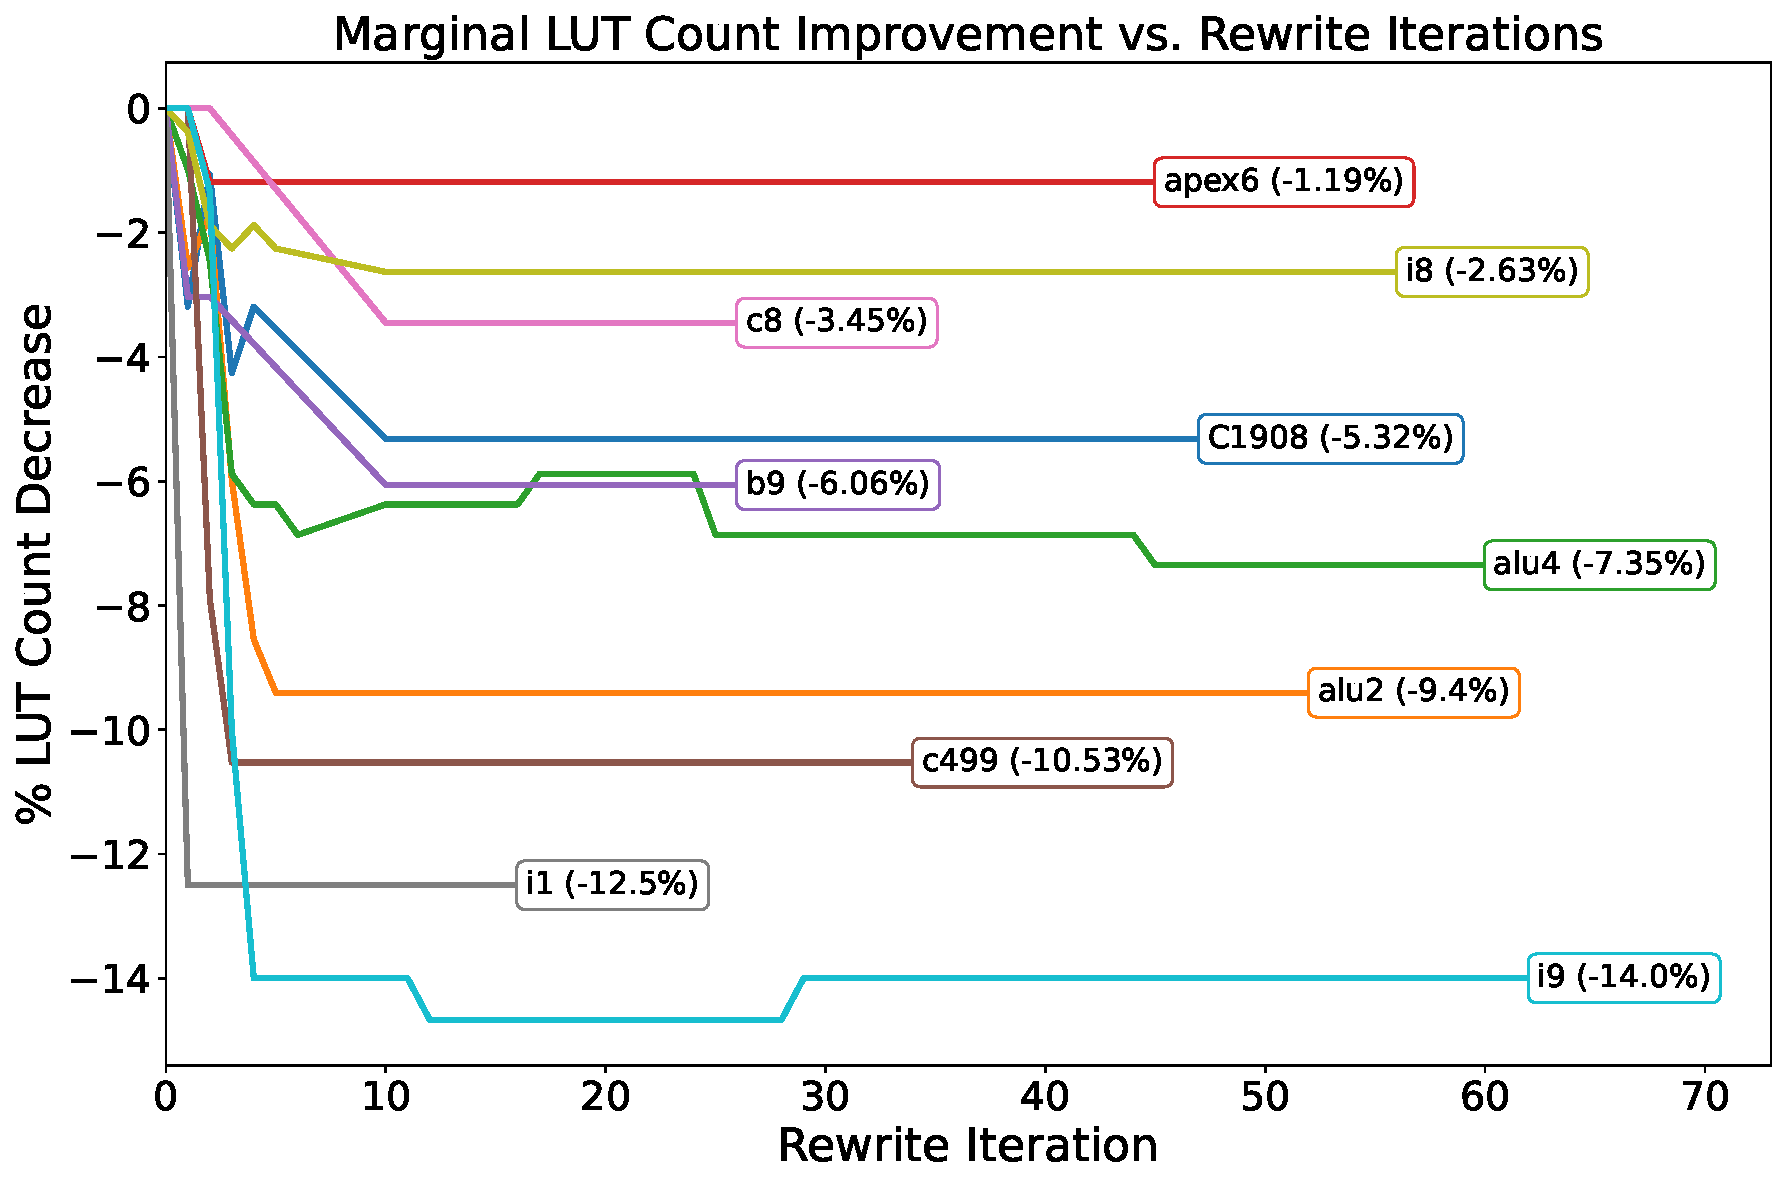
\includegraphics[width=\textwidth]{img/improvement.pdf}
        \caption{Marginal improvement in LUT count versus iteration count. The labels mark equality saturation.}\label{fig:marginal:improvement}
    \end{subfigure}
    \hfill\vspace{4mm}
    \begin{subfigure}{0.47\textwidth}
        \centering
        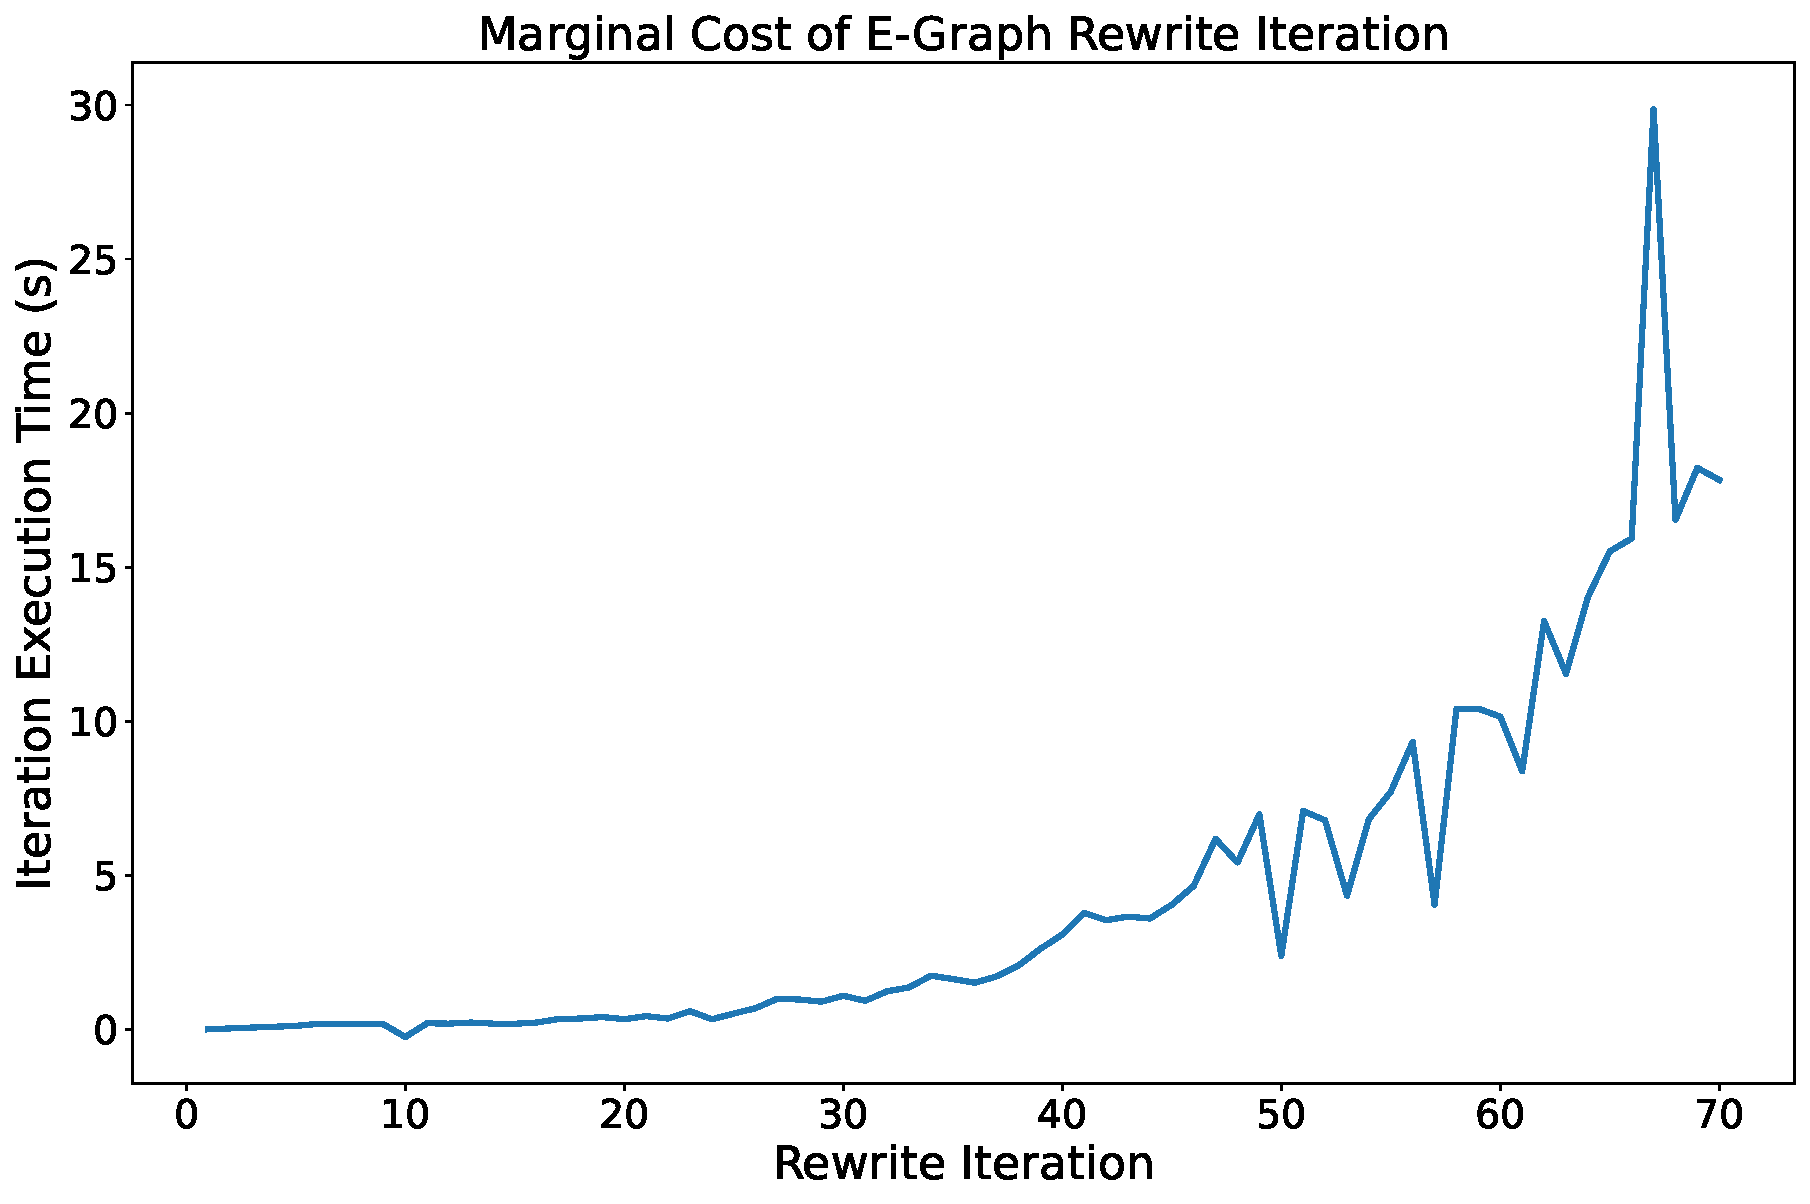
\includegraphics[width=\textwidth]{img/runtime_derivative.pdf}
        \caption{Marginal cost in compile time versus iteration count. Later iterations consume more time as the e-graph is larger.}\label{fig:marginal:runtime}
    \end{subfigure}
    \caption{The marginal gain in QoR and cost in time as the e-graph grows in size. In most cases, exploring a circuit to equality saturation is not necessary.}\label{fig:marginal}
\end{figure}

\begin{table*}[t]
    \centering
    \caption{Post-implementation results of pipelined multiplication circuit optimized with EqMap. Yosys 0.33 + EqMap is used for synthesis, and Vivado 2024 is used for placement and routing.}\label{tab:multiply}
    \csvreader[
        tabular=lrrrrrrrrr, % Custom alignment for this instance
        late after line=\\, % Add \\ after each row
        late after last line=\\ \bottomrule, % Prevent extra \\ after the last row
        table head=\toprule $\times$ Num. Stages & LUTs & & & Depth & & & CLBs & & \\ \midrule
    ]{data/mult.csv}{1=\one, 2=\two, 3=\three, 4=\four, 5=\five, 6=\six, 7=\seven, 8=\eight, 9=\nine, 10=\ten}%
    {\one & \two & \three & \four & \five & \six & \seven & \eight & \nine & \ten}
\end{table*}

\subsection{Marginal Gain and Cost}\label{sec:results:margin}

Given that \shortname{} is fundamentally a superoptimization tool, we want to
provide evidence that significant gains can be found within reasonable time
bounds. To that end, we empirically studied the marginal gains in QoR as
increasingly longer rewrite sequences are added to the e-graph. Within the
e-graph infrastructure, this phasing of applying rewrites and rebuilding the
union-find data structure is referred to as an \textit{iteration}. As shown in
Fig.~\ref{fig:marginal:improvement}, nearly all the performance gains are
discovered within the first 10 iterations---well before equality saturation.
Some notable exceptions occur, such as `alu4' being reduced in size after the
40th iteration. Lastly, the growing runtime of e-graph exploration with each
iteration should be addressed. The marginal cost of executing an iteration of
rewrites becomes prohibitive as the e-graph becomes larger.
Fig.~\ref{fig:marginal:runtime} illustrates that after approximately the 30th
iteration, the added cost in compile time rapidly increases. However, the far
majority of results are reached within 20 iterations of rewriting, which on
average takes only 3 seconds.

\subsection{Case Study: Pipelined Designs}\label{sec:results:retiming}

Hardware designs with feed forward pipelines provide interesting opportunities
to find a higher-level of area optimization. When closing timing on FPGA
designs, the critical path is often dominated by routing, more so than ASIC
design. Hence, reducing the cell count and circuit depth along the max delay
path is a valid optimization strategy for FPGA design. As a caveat, it is
important to note that other work has also observed the opposite
trend~\cite{academicfpga}: decreasing depth too much can strain the router. In
any case, \shortname{} can be utilized to reduce total CLB usage in pipelined
designs. To test this hypothesis, our compiler was used to optimize a 32-bit
integer multiplier with a varying number of pipeline stages. The data in
Table~\ref{tab:multiply} clearly shows that as the number of pipeline stages
increases, an inefficiency in the mapping is accumulated. \shortname{} is able
to repack the LUTs into roughly the same amount of logic as the single stage
design---without increasing the number of flip-flops. While our current
technique only supports acyclic designs, we wanted to add an additional case
study on a pipelined operator to prove the potential of extending our approach
beyond combinational logic.

While the drop in CLB usage is desirable, we anticipate that more exact
extraction techniques would find even greater area reductions. Unlike other
logic rewrites, register retiming changes the topology of the stateful
elements---i.e. the flip-flops. Consequently, greedy extraction cannot take
into account the fan-out these flip-flops. While these results \textit{do}
demonstrate that optimizing for CLB count over raw cell count is a feasible
strategy, a different extraction method will be needed.

\subsection{Case Study: Bit-Parallel Designs}\label{sec:results:scalability}

While the academic benchmarks enable direct comparisons to the rest of the
literature, the circuits are relatively small. On average, the designs map to
670 LUTs. Among the \nimproved{} improved benchmarks in
Table~\ref{tab:results}, only six exceed 1000 LUTs. Although this e-graph
driven technology provides promising results for smaller benchmarks, FPGA
technology mapping is especially difficult---and important---for larger designs
with tens of thousands of LUTs. Through our case study on bit-parallel designs,
we demonstrate that \shortname{} performs just as well on large designs,
achieving area reductions without incurring excessive build times.

To test how \shortname{} scales with increasing numbers of LUTs, we created a
synthetic ALU benchmark and varied the input and output bit widths from 8 bits
to 4096 bits. Table~\ref{tab:alu} lists the LUT counts from the initial
synthesis by Vivado 2024, followed by the packed LUT counts. Even though the
1024-bit, 2048-bit, and 4096-bit ALU designs had up to 15,000 LUTs,
\shortname{} was able to achieve up to almost 15\% improvement over Vivado
within 5 minutes of extra build time. While longer runs lead to slightly better
improvements, these results demonstrate how \shortname{} can achieve area
reductions within a short period of time, even when input designs are scaled to
beyond 10,000 LUTs. In this specific case, \shortname{} can be used to audit
synthesis tools and perhaps even reverse-engineer adverse behavior. Hence,
\shortname{} proves to be a practical tool to run after a baseline synthesis by
Vivado or Yosys to quickly achieve better LUT packing with minimal time cost.

\begin{table}
    \centering
    \caption{EqMap synthesis results of $n$-bit ALU}\label{tab:alu}
    \csvreader[
        tabular=lrrr, % Custom alignment for this instance
        late after line=\\, % Add \\ after each row
        late after last line=\\ \bottomrule, % Prevent extra \\ after the last row
        table head=\toprule ALU Bit Width & LUT Count &  &  \\ \midrule
    ]{data/alu.csv}{1=\Name, 2=\LC, 3=\City, 4=\Thing}%
    {\Name & \LC & \City & \Thing}
\end{table}
\section{Conclusion and Future Work}\label{sec:conclusion}
While technology mapping has been studied for decades, the end of transistor
scaling will require new logic synthesis tools that are less heuristic in
nature. This work seeks to demonstrate that there are practical solutions that
can bridge the gap between SAT-based exact synthesis and cut enumeration
techniques. With \shortname{}, we can use e-graphs to improve FPGA technology
mapping with a post-processing compilation step. Specifically, our results show
that \shortname{} improves synthesis by \metric{} on average without increasing
circuit depth. While other techniques may approach or beat these gains,
equality saturation as a formal method makes e-graphs a particularly
trustworthy method by which to transform circuits. Lastly, e-graph construction
is decoupled from extraction, meaning this type of flow is particularly
adaptive to new optimization objectives.

As for future work, the main research problem is the integration of more
sophisticated extraction techniques. The final QoR is still largely contingent
on e-graph extraction, and more advanced extraction techniques would likely
improve the results even further. While simple greedy extraction clearly serves
a purpose, it fails to capture the full potential of \shortname{}'s rewriting
system. Nonetheless, \shortname{} is a promising step towards EDA tools that
can better span the gap between exact and fully heuristic logic synthesis.


% Unstarted sections:
% [ ] Mult results: a big opportunity, but greedy extraction somewhat ruins it
% [ ] Future work

% Unstarted figures:
% [ ] A rewritten circuit (re-make by hand)

% MISC TODOS:
% (Matt): Explain the bumps and dips in the plot
% (Matt): Explain somewhere (prob results) that iterations/time *sometimes* mattter
% (Matt): Explain/mention rewrite figure in text

% use the ACM bibliography style
\bibliographystyle{ACM-Reference-Format}
\bibliography{references}

% \newpage
%%
%% If your work has an appendix, this is the place to put it.
% \appendix

\end{document}